\chapter{Manual de usuario}
\label{manualusuario}

\section{Requerimientos}

Si bien el sistema desarrollado se ha probado en sistemas Linux y Windows, a continuación se enumera los programas y librerías necesarias para una instalación en el sistema operativo Ubuntu 14.04.
\begin{itemize}
\item Instalar \textit{ Matlab R2011b}.
\item Desde el repositorio local los siguientes paquetes:
	\begin{itemize}
		\item \texttt{matlab-support}
		\item \texttt{matlab-support-dev}
	\end{itemize}
\item	\textit{OpenCV} desde librerías del repositorio local:
	\begin{itemize}
		\item libcv-dev
		\item libopencv-dev
	\end{itemize}
\item Instalar \textit{cvblob}\cite{cvblob}. Descargar \texttt{cvblob-0.10.4-src.tgz} y seguir  el instructivo de la página para una instalación Linux.
\item Copiar la carpeta del proyecto \texttt{Proyecto\_Biomecanica}.
\item Compilar el programa que efectúa la segmentación. Para ello ir a la carpeta \texttt{Proyecto\_Biomecanica/segmentacion} y crear una carpeta \texttt{/build}.
Dentro de ella abrir una terminal y ejecutar:
\begin{center}
\begin{tabular}{l}
\texttt{cmake ..}\\
\texttt{make   }
\end{tabular}
\end{center}

A continuación en \texttt{Proyecto\_Biomecanica/segmentacion/build/client} se tiene el ejecutable con el nombre \texttt{Source}, el mismo se debe llevar a la carpeta \texttt{Proyecto\_Biomecanica/SISTEMA/ProgramaC} con el nombre \texttt{Source\_GLNX86} si se instalo un sistema de 32 bits o \texttt{Source\_GLNXA64} en caso contrario.

\item Instalar \textit{Blender} desde los repositorios locales.
\end{itemize}


\section{Generación de secuencias sintéticas}

A continuación se resumen los pasos a seguir para generar una secuencia en el laboratorio virtual a partir de archivos BVH de la base de datos \textit{MotionBuilder-friendly version} ofrecidas por \textit{cgspeed} \cite{cgspeed}, 
%\footnote{\textcolor{blue}{\underline{\url{https://sites.google.com/a/cgspeed.com/cgspeed/motion-capture}}}. Accedido 4-12-14},
 que provienen de las capturas de Carnegie Mellon University Motion Capture Database \cite{CMU}. La secuencia generada se almacena en la base de datos del proyecto.
 
 \begin{enumerate}
 \item Seleccionar el movimiento que va a tener la secuencia, se tiene una  lista disponible en \textit{cgspeed}\footnote{{\tiny \textcolor{blue}{\underline{\url{https://sites.google.com/a/cgspeed.com/cgspeed/motion-capture/cmu-bvh-conversion/bvh-conversion-release---motions-list}}}}. Accedido 4-03-15}. 
 \item Preparar la secuencia. Para ello se utiliza el programa bvhacker\footnote{Se ha probado la versión 1.8.0.6 sobre wine 1.6.2 simulando este último a Windows XP} \cite{bvhacker}, al abrir la secuencia se quita el offset y se efectúa un centrado de la misma, con las opciones \texttt{NoOffset} y \texttt{Center} respectivamente, luego se guarda convenientemente \texttt{File/Save}.
 \item Activar la importación de archivos BVH en el menú de preferencias del entorno \textit{Blender}, \texttt{File/User\_Preferences/Addons/Import-Export\_bvh}.
 \item Crear las carpetas correspondientes en la base de datos. Para ello correr el script \texttt{Base\_de\_datos/nueva\_secuencia.sh }. Dicho script de \texttt{Bash} ejecuta dentro de \textit{Blender} los script \texttt{import\_bvh.py} y \texttt{acoplar\_modelo.py}, que permiten respectivamente importar el archivo BVH previamente preparado y acoplarlo con el modelo y los marcadores.
 \item Abrir el archivo .blend de la nueva secuencia  y efectuar los ajustes finos del modelo virtual sobre el esqueleto. El modelo virtual se encuentra en el \texttt{layer 1}, los marcadores en el \texttt{layer 2}  y el esqueleto en el \texttt{layer 3}. Solo se debe modificar el modelo virtual.
 \item Por último para renderizar la secuencia del laboratorio virtual, se debe seleccionar apropiadamente las propiedades de las cámaras en el menú\\ \texttt{Properties/Render}, seleccionar únicamente el \texttt{layer 1} y el \texttt{layer 2} con el modelo virtual y los marcadores para que sean  visibles en pantalla y luego abrir en el editor de texto de \textit{Blender} el script \texttt{render.py} y ejecutarlo. De esta manera automáticamente se generan y almacenan los videos en la estructura de datos de la base de datos.
 
 \end{enumerate}
 
 \section{Procesamiento de datos utilizando interfaz gráfica}
 
 Una vez abierto \textit{Matlab} con el workspace en \texttt{/Proyecto\_Biomecanica/SISTEMA}, se debe ejecutar el script \texttt{main.m}. El mismo se encarga de cargar los \texttt{paths} necesarios, abrir \texttt{matlabpool}\footnote{Por defecto Matlab utiliza 2 núcleos del procesador, si se desea configurar un número mayor de núcleos se debe acceder a \texttt{/Parallel/Manage\_Configurations} } para utilizar múltiples procesadores y mostrar la interfaz de usuario.
 
 
 La interfaz se divide en 6 zonas principales:
 \begin{enumerate}
 \item Basic configuration
 \item Segmentation
 \item Reconstruction
 \item Tracking
 \item Blocks
 \item Process Data, View Data
 \end{enumerate}
 
 \begin{figure}[ht!]
 \hspace{-1cm}
 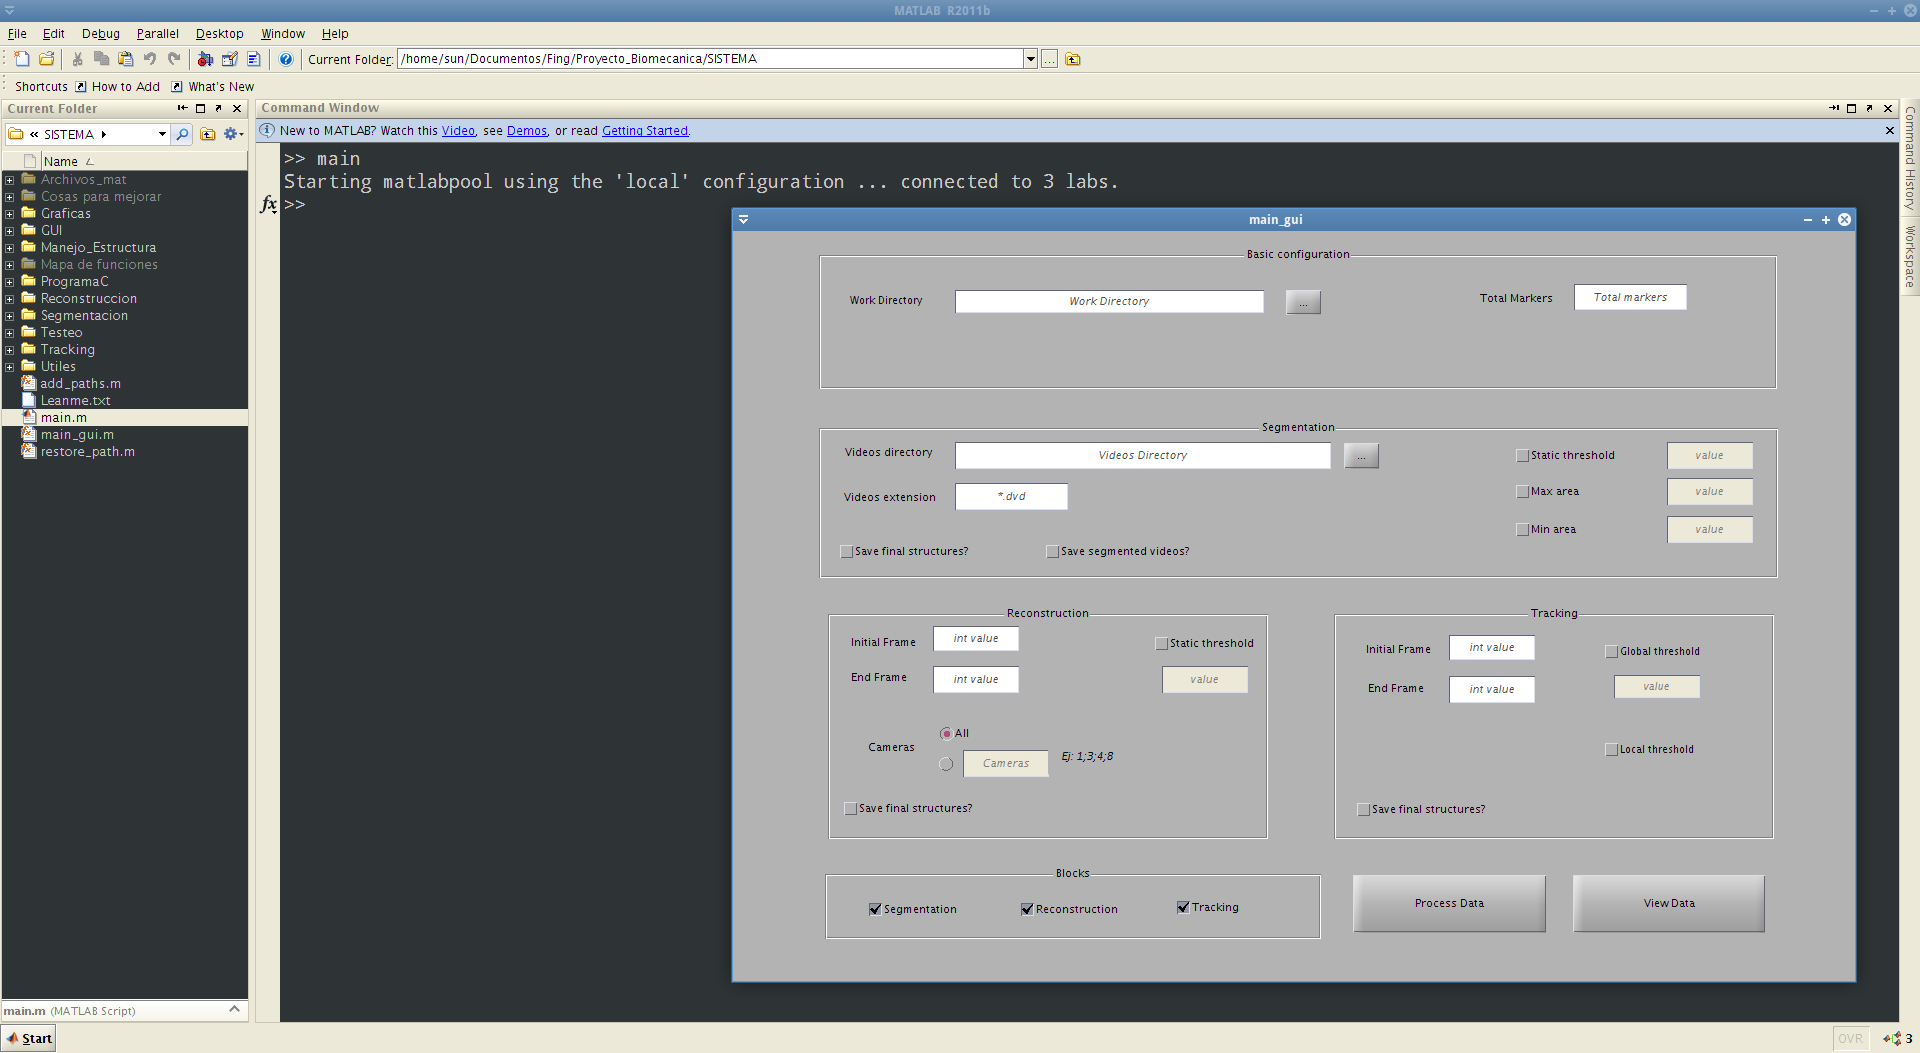
\includegraphics[scale=0.23]{img/Manual_de_usuario/main.png}
 \caption{Resultado de \texttt{main.m} en \textit{Matlab}.}
 \label{fig:main.m}
 \end{figure}
 
 \subsection{Basic configuration}
 Los parámetros a ingresar son:
 \begin{itemize}
  \item \texttt{Work Directory} es el directorio donde se almacena la información de los datos procesados. En el caso de trabajar con la base de datos por ejemplo para la secuencia sintética del sujeto 09\_07 con videos de resolución 1600x600 y los cuadros por segundo del bvh original, la carpeta a seleccionar es:\\ \texttt{Base\_de\_datos/Sujeto\_CMU\_09/09\_07/Datos\_Procesados/1600\_600-100-100}.
  \item \texttt{Total Markers} indica al sistema el número de marcadores utilizados. Dicho número se utiliza sobre todo en las etapas de reconstrucción y seguimiento. En la versión actual del sistema es recomendable, si la secuencia tiene $n$ marcadores, ingresar un valor de al menos $n+2$, para evitar perdida de  marcadores en reconstrucción.   
 \end{itemize}
 
 \subsection{Segmentation}
 \begin{itemize}
   \item \texttt{Videos Directory} es el directorio donde se deben encontrar los videos a procesar. En el caso de trabajar con la base de datos por ejemplo para la secuencia sintética del sujeto 09\_07 con videos de resolución 1600x600 y los cuadros por segundo del bvh original, la carpeta a seleccionar es:\\ \texttt{Base\_de\_datos/Sujeto\_CMU\_09/09\_07/Datos\_Imagen/1600\_600-100-100}.
   \item \texttt{Videos extension}, casilla que permite ingresar la extensión de los videos a procesar, por defecto se utiliza la extensión .dvd que es un tipo de archivo mpeg. 
   \item \texttt{Save final structures}. Se debe seleccionar esta casilla si se desea obtener archivos .mat y .xml de las estructuras  cam y skeleton, dentro de la carpeta  de trabajo ingresada (\texttt{Work Directory/<Resolución>/Segmentacion}).
   \item \texttt{Save segmented video}. Esta casilla permite guardar  los videos que resultan de la salida de los bloques de umbralización y detección de blobs del último video segmentado. De esta manera si puede visualizar las distintas etapas de la segmentación y ajustar manualmente los parámetros de entrada en caso de ser necesario. Los videos de salida se almacenan en la carpeta de los videos a segmentar (\texttt{Videos Directory}).
   \item \texttt{Static threshold} es un parámetro opcional. El mismo establece un umbral fijo para la umbralización, debe ser un valor entre 0 y 255.
   \item \texttt{Max area} es un parámetro opcional que modifica el área máxima del filtrado por área. Debe ser un valor positivo.
   \item \texttt{Min area} es un parámetro opcional que modifica el área mínima del filtrado por área. Debe ser un valor positivo.
  \end{itemize}
 \subsection{Reconstruction}
 \begin{itemize}
    \item \texttt{Init Frame}, se ingresa el cuadro a partir del cual se efectúa la reconstrucción. 
    \item \texttt{End Frame}, se ingresa el cuadro final hasta el cual se efectúa la reconstrucción. 
    \item \texttt{Cameras}. Por defecto se reconstruye con todas las cámaras disponibles en la estructura cam sobre la cual se está trabajando, si se desea hacer reconstrucciones con cierto conjunto de cámaras se debe seleccionar la segunda casilla e ingresar el conjunto de cámaras.
    \item \texttt{Save final structures}. Se debe seleccionar esta casilla si se desea obtener archivos .mat y .xml de las estructuras  cam y skeleton, dentro de la carpeta  de trabajo ingresada (\texttt{Work Directory/<Resolución>/Reconstruccion}).
    \item \texttt{Static threshold} es un parámetro opcional. El mismo establece un umbral máximo dentro del cual buscar validaciones de una posible  reconstrucción, el valor se debe ingresar en metros.
   \end{itemize}
 
  \subsection{Reconstruction}
  \begin{itemize}
     \item \texttt{Init Frame}, se ingresa el cuadro a partir del cual se efectúa el seguimiento. 
     \item \texttt{End Frame}, se ingresa el cuadro final hasta el cual se efectúa seguimiento.      
     \item \texttt{Save final structures}. Se debe seleccionar esta casilla si se desea obtener archivos .mat y .xml de las estructuras  cam y skeleton, dentro de la carpeta  de trabajo ingresada (\texttt{Work Directory/<Resolución>/Tracking}).
     \item \texttt{Global threshold} es un parámetro opcional para efectuar pruebas sobre el algoritmo de seguimiento.
     \item \texttt{Local threshold} es un parámetro opcional para efectuar pruebas sobre el algoritmo de seguimiento. 
   \end{itemize}
   
    \begin{figure}[ht!]
    \hspace{-1cm}
    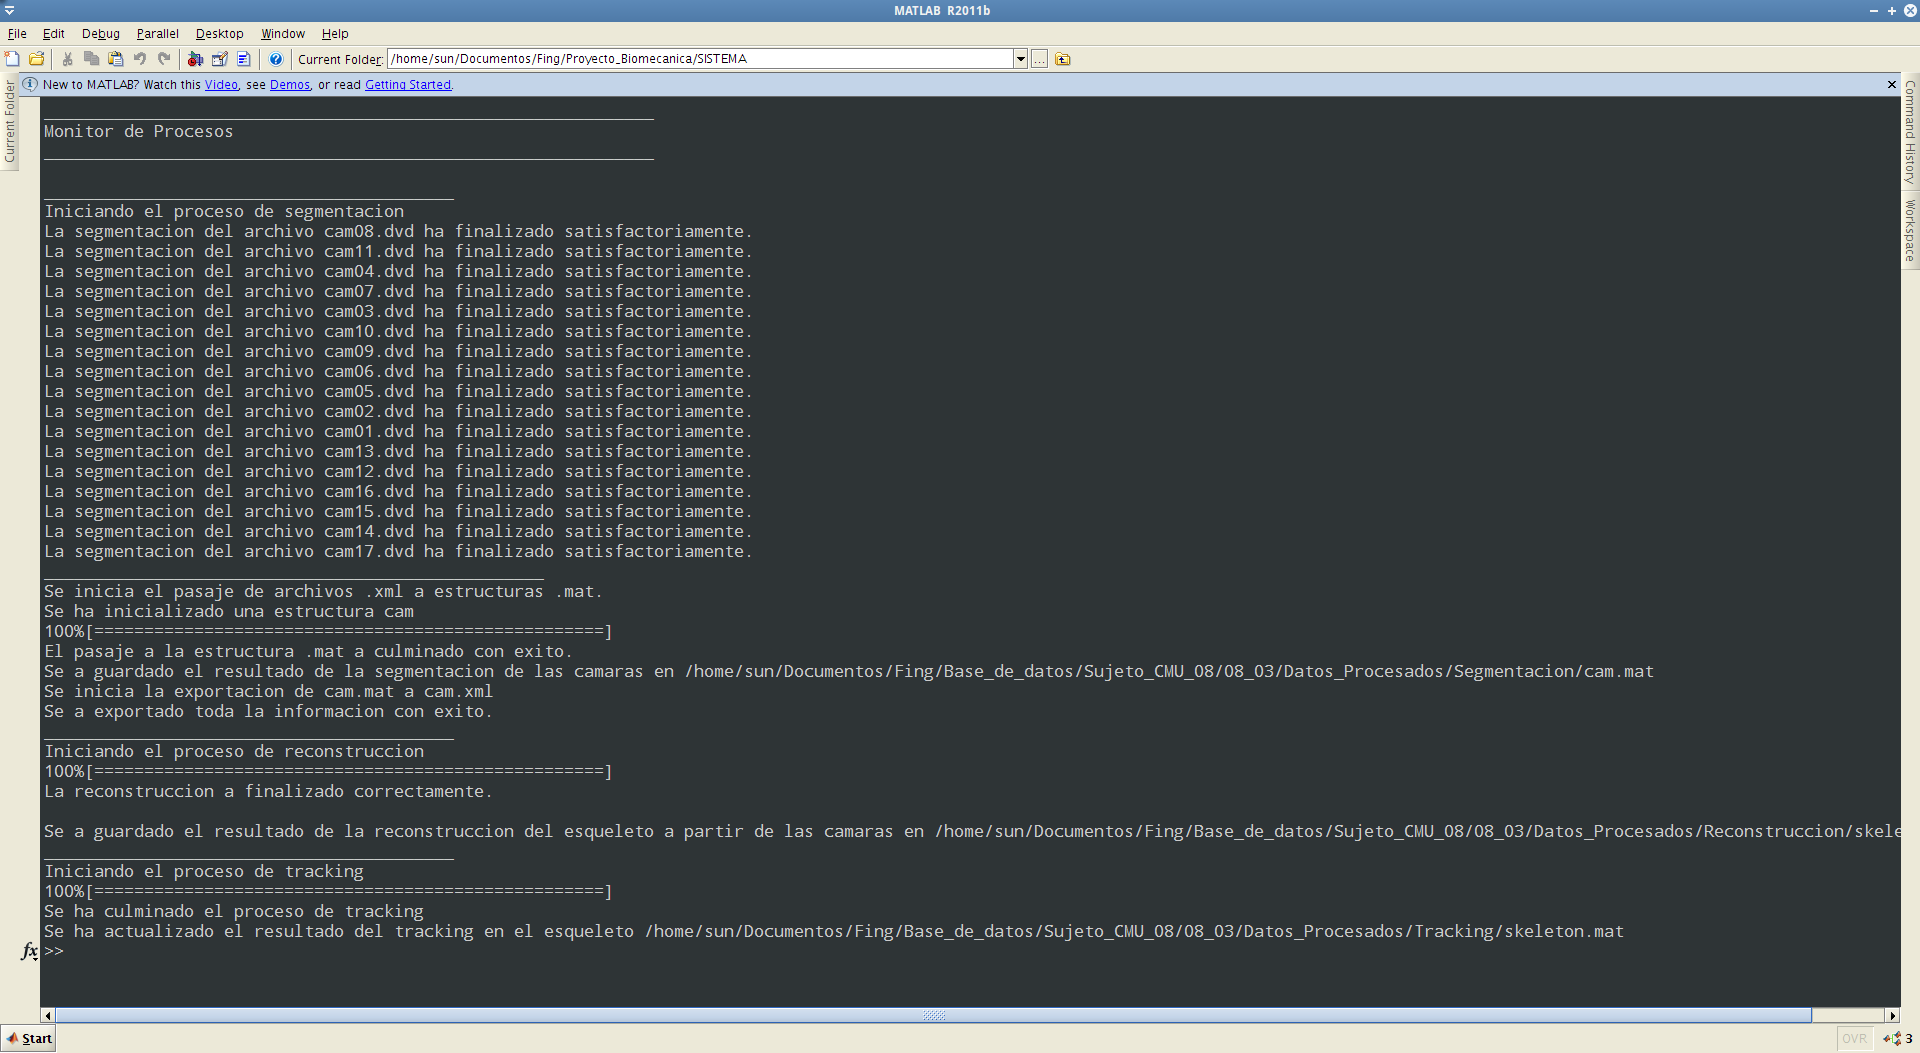
\includegraphics[scale=0.23]{img/Manual_de_usuario/resultados_procesamiento.png}
    \caption{Resultados del procesamiento en la consola de \textit{Matlab}.}
    \label{fig:main.m}
    \end{figure}
   
 
 \section{Bugs}

 
 En Ubuntu 14.04 de 32 bits, cuando se ejecuta la segmentación desde la interfaz gráfica la primera vez que se abre \textit{Matlab}, en algunas oportunidades no se carga correctamente el ejecutable \texttt{Source\_GLNX86}. Los pasos a seguir para solucionar este inconveniente son:
 \begin{itemize}
 \item Verificar que el ejecutable funcione fuera de Matlab. Abrir una terminal donde se encuentre el ejecutable y ejecutar:
 \begin{center}
 \texttt{./Source\_GLNX86} \hspace{0.05cm}   \texttt{<vidpath>}
 \end{center} donde \texttt{<vidpath>} es la dirección del video a segmentar.
 \item Si en el paso anterior no funciona la segmentación, compilar nuevamente el programa que efectúa la segmentación, revisar si dicha compilación finaliza correctamente y colocar el ejecutable en\\ \texttt{Proyecto\_Biomecanica/SISTEMA/ProgramaC} con el nombre \texttt{./Source\_GLNX86}. En caso que si funcione la segmentación en la terminal, entonces el problema es de \textit{Matlab}. Una solución es ejecutar tres veces la segmentación desde la interfaz gráfica, cuidando antes de cada ejecución de tener el workspace \textit{Matlab} en \texttt{/Proyecto\_Biomecanica/SISTEMA}. A la tercera vez el sistema funcionará, y de ahí en más mientras se tenga abierto \textit{Matlab} se ejecuta todo normalmente.
 \end{itemize}
  